\documentclass[./thesis.tex]{subfiles}
\begin{document}
\chapter{Coinductive types in univalent type theory}
\label{chap:coinductive-types-in-univalent-type-theory}

The results in this chapter mainly appear in the \UniMath{} package
\unimathname{Induction}, so that prefix is left off
(e.g.\ \unimathname{Induction.W.Core} is shortened to
\unimathname{W.Core}).

\section{W and M}
\label{sec:w-and-m}

Per Martin-Löf introduced W-types as a way to study types with a well-ordering.
In fact, W-types provide a general and convenient setting for the study of
induction. In extensional type theories, W-types are initial algebras (as in
\cref{def:initial-alg}) for polynomial functors (see
\cref{def:polynomial-functor}), so all the examples we've seen so far of
inductive types defined as functor algebras are W-types.

Dually, M-types are
non-wellfounded trees, that is, trees with potentially infinitely long branches.

\begin{definition}\label[definition]{def:container}
  A \define{container}\index{Container} (sometimes called a
  \define{signature}\index{Signature} by analogy, see
  \cref{rmk:universal-algebra}) is a pair $(A,B)$ of a type
  $A:\universe$ and a family $B:A→\universe$.
\end{definition}
Given a container, we can form the associated W- and M-types:
\begin{align*}
  \prftree[r]{}
    {Γ ⊢ A:\universe}{Γ ⊢ B:A\to\universe}
    {Γ ⊢ \type{\W{a}{A}{B}}}
  &&
  \prftree[r]{}
    {Γ ⊢ A:\universe}{Γ ⊢ B:A\to\universe}
    {Γ ⊢ \type{\M{a}{A}{B}}}
\end{align*}
These types are shaped like trees. An element of a W-type is specified by
an element $a:A$ (the ``label'' of this vertex) and a function
$b:\apply{B}{a}\to \W{x}{A}{B}$ which picks out its subtrees.
\begin{equation*}
  \prftree[r]{}
    {Γ ⊢ a:A}
    {Γ ⊢ b:B(a)\to \W{x}{A}{B}}
    {Γ ⊢ \sup{a}{b}:\W{x}{A}{B}}
\end{equation*}
Martin-Löf points out that a ``bottom'' or ``leaf'' element can be given by
taking one of the $\apply{B}{a}$ to be $\emptytype$ and the subtree-function to
be the one provided by $\rec_{\emptytype}$ (example in
\cref{ex:nat-w})\cite{martin-lof-itt}.

The typographically-challenging elimination rule\index{Elimination!For W-types}
for W-types encodes transfinite induction. If, when a property
$C:\W{a}{A}{B}→\universe$ holds for all subtrees of a given node it also holds
for that node, then it holds for any element in $\W{a}{A}{B}$:
\begin{equation*}
  \prftree[r]{}
    {Γ ⊢ w:\W{a}{A}{B}}
    {\prftree[r, noline]{}
      {Γ,\quad a:A,\quad f:\apply{B}{a}→\W{a}{A}{B},\quad g:\∏{b:\apply{B}{a}}{\apply{C}{(\apply{f}{b})}}}
      {⊢\apppply{h}{a}{f}{g}: C(\sup{a}{f})}}
    {Γ ⊢ \appply{\recW}{w}{h}:\apply{C}{w}}
\end{equation*}
As a function:
\begin{multline*}
	\recW : \∏{C:\W{a}{A}{B}→\universe}{}
  \paren{\∏{a:A}{\∏{f:\apply{B}{a}→\W{a}{A}{B}}
                    {\∏{g:\∏{b:\apply{B}{a}}{\apply{C}{(\apply{f}{b})}}}{\apply{C}{(\sup{a}{f})}}}}}
                \\ →\∏{w:\W{a}{A}{B}}{\apply{C}{w}}
\end{multline*}

\begin{example}\label[example]{ex:nat-w}
  The natural numbers are readily encoded as a W-type.
  Define $B\defeq \apppply{\rec_{\booltype}}{\universe}{\emptytype}{\unittype}$
  so that $\apply{B}{\bfalse}\jdeq \emptytype$ and
  $\apply{B}{\btrue}\jdeq\unittype$, and consider $\N'\jdeq \W{b}{A}{B}$.
  Let $!$ be the unique function out of the empty type and further define:
  \begin{align*}
    \begin{split}
      0_{\N'} &: \W{b}{\booltype}{B} \\
      0_{\N'} &\defeq \sup{\bfalse}{!} \\
    \end{split}
    \begin{split}
      1_{\N'} &: \W{b}{\booltype}{B} \\
      1_{\N'} &\defeq \sup{\btrue}{(\λ{x}{0_{\N'}})}
    \end{split}
  \end{align*}
  Following this pattern, we can define
  \begin{align*}
    \suc &: \N' \to \N' \\
    \suc &\defeq \λ{n}{\sup{\btrue}{(\λ{x}{n})}}
  \end{align*}
  so that $1_{\N'}\equiv \apply{\suc}{0_{\N'}}$. What does this tree look like?
  Well, by virtue of construction, $0_{\N'}$ is its least element. Applying
  $\suc$ gives us an element at one level higher in the tree than the one we put
  in.
  \vspace{-2em}\begin{center}
    \begin{tikzpicture}[scale=4]
      \node (A) [scale=2] {$\cdot$};
      \node     [above of=A] {$0_{\N'}$};

      \node (B) [scale=2, right of=A] {$\cdot$};
      \node     [above of=B] {$1_{\N'}$};

      \node (C) [scale=2, right of=B] {$\cdot$};
      \node     [above of=C] {$\apply{\suc}{1_{\N'}}$};

      \node (D) [scale=2, right of=C] {$\cdot$};
      \node     [above of=D] {$\cdots$};

      \node     [right of=D, scale=2.0, color=white] {$\cdot$};
      \node (E) [right of=D, xshift=1cm] {$\cdots$};
      \node     [scale=2, above of=E, color=white] {$\cdots$};

      \draw[->] (A) edge (B);
      \draw[->] (B) edge (C);
      \draw[->] (C) edge (D);
      \draw[->] (D) edge (E);
      % \draw (A) edge [in=-60,out=-20,loop] node[below] {$e$} (A);
    \end{tikzpicture}
  \end{center}

  We can derive from the induction principle of $\booltype$ that it
  only has two elements, $\bfalse$ and $\btrue$ \TODO{reference}.
  Using this (and ignoring uniquely specified terms like $!$),
  the W-elimination rule for $\N'$ can be reshaped and simplified:
  \begin{equation*}
    \prftree[r]{}
      {Γ ⊢ n:\N'}
      {\prftree[r, noline]{}
        {Γ⊢h_1: C(0_{\N'})}}
      {\prftree[r, noline]{}
        {Γ, f:\unittype→\N',g:\∏{\unitelem:\unittype}\apply{C}{(\apply{f}{\unitelem)}}}
        {⊢\appply{h_2}{f}{g}: \apply{C}{(\sup{\btrue}{f})}}}
      {Γ ⊢ \apppply{\rec_{\N'}}{n}{h_1}{h_2}:\apply{C}{n}}
  \end{equation*}
  But since a function $\unittype→\N'$ is equivalent to picking out a single
  element of $\N'$ and $\sup{\btrue}{f}\equiv\apply{\suc}{f}$,
  this is just the elimination rule for the natural numbers (\cref{def:nat})
  in disguise.
\end{example}

Other examples include lists, binary trees, ordinals of the second number
class, and more.\TODO{reference} In the next few sections, we will develop a
correspondence between W-types (resp.\ M-types) and initial algebras (resp.\
terminal coalgebras) for a general class of functor on $\universe$, which will
include all examples in \cref{sec:functors-and-their-algebras}.

\section{Preliminaries}
\label{sec:preliminaries}

\begin{definition}[\unimathname{PolynomialFunctors.polynomial\_functor}]
  \label[definition]{def:polynomial-functor}
  Given a container $S\defeq (A,B)$, its associated \define{polynomial functor}
  is the function
  \begin{gather*}
    P_{A,B}:\universe\to \universe \\
    \apply{P_{A,B}}{X}\defeq\∑{a:A}{B(a)\to X}
  \end{gather*}
  We will regularly leave off the subscript for $P$.
  The \define{action} of $P$ on functions is
  \begin{gather*}
    P^* : (X\to Y)\to P_{A,B}(X)\to P_{A,B}(Y) \\
    \apply{P^*f}{(a,g)}\defeq (a,g∘f).
  \end{gather*}
\end{definition}

\begin{remark}
	Technically, polynomial functors aren't functors, since $\universe$ isn't
  a category (the whole point of the univalent perspective is that it behaves
  more like a weak higher category). It has functorial properties only up to
  \textit{propositional} equality (as in \cref{def:functor-tt}), which will
  suffice for the following proofs. That is, we have
  \begin{align*}
    \apply{P^*}{(g∘f)} = \apply{P^*}{g}∘\apply{P^*}{f}
    &&
    \apply{P^*}{\id_X} = \id_{\apply{P}{X}}
  \end{align*}
\end{remark}

\begin{definition}\label[definition]{def:algebra-coalgebra-in-utt}
  Exactly as in \cref{def:f-coalgebra}, we define the type of (co)algebras for a
  polynomial functor $P$ associated to a container $(A,B)$ as follows:
  \begin{align*}
    \Algtype_P\≔\∑{A:\universe}{PA→A} && \Coalgtype_P\≔\∑{A:\universe}{A→PA}
  \end{align*}
  and coalgebra morphisms as
  \begin{align*}
    \ttfun{CoalgMor}((X,α),(Y,β))
    &\≔ (X,α)⇒(Y,β) \\
    &\≔ \∑{f:X→Y}{(\apply{P}{f})∘α = β∘f}
  \end{align*}
  with algebra morphisms defined dually \cite{homotopy-initial}.
\end{definition}

See \cref{ex:nat-functor-utt} for the polynomial functor for which $\ℕ$ is
initial.

\section{Uniqueness}
\label{sec:uniqueness}

Fix a container $S\defeq (A,B)$ and let $P$ be the associated polynomial functor.
We will prove a few auxiliary lemmas on the way to the following result.
This proof appeared in the \Agda{} formalization of \cite{non-wellfounded}, this
is its first appearance ``de-formalized''.

\begin{lemma}[\unimathname{M.Uniqueness.M\_coalg\_eq},
              \unimathname{M.Uniqueness.isaprop\_M}]
  \label[lemma]{lemma:terminal-colagebra-unique}
  Any two terminal $P$-coalgebras are equal. In other words, the following type is
  a proposition:
  \begin{equation*}
    \apply{\Final}{\dpair{A}{B}}\defeq
    \∑{(X,α):\apply{\Coalgtype}{\dpair{A}{B}}}{
      \∏{(Y,β):\apply{\Coalgtype}{\dpair{A}{B}}}
        {\apply{\isContr}{\dpair{Y}{β}⇒\dpair{X}{α}}}
    }
  \end{equation*}
\end{lemma}

First, we'll show that their carriers are equivalent:

\begin{lemma}[\unimathname{M.Uniqueness.M\_carriers\_iso}]
  \label[lemma]{lemma:algebra-iso-equiv}
	If $(X,α)$ and $(Y,β)$ are terminal $P$-coalgebras,
  then the first projections of the unique coalgebra morphisms
  $f:X⇒ Y$ and $g:Y⇒ X$ induce
  an equivalence of types $\weq{X}{Y}$.
\end{lemma}

The proof is standard category theory, namely that two objects
satisfying the same universal property are isomorphic
(compare to \cref{lemma:terminal-unique}).

We can then invoke the characterization of paths in Σ-types,
\cref{lemma:path-sigma}. We'll need to demonstrate that the coalgebra map
$α:X\to FX$ is equal to $β:Y\to FY$ when transported along the path
constructed in \cref{lemma:algebra-iso-equiv}.

\begin{lemma}\label[lemma]{lemma:polynomial-functor-transport}
  For all $X,Y:\universe$, $F:\universe\to\universe$,
  $f:X\to FX$, $g:Y\to FY$, and $p:\propeq{}{X}{Y}$,
  if for all $x:X$ we have
  \begin{equation*}
    \propeq{}{
      \transport{F}{p}{(\apply{f}{x})}
    }{
      \apply{g}{({\transport{\id_{\universe}}{p}{x}})}
    }
  \end{equation*}
  then $\propeq{}{\transport{Z↦ (Z\to FZ)}{p}{f}}{g}$.
  That is, $f$ is equal to $g$ after being transported just when
  applying $f$ and transporting the result is the same as transporting the
  input and applying $g$.\footnote{This is a corollary of Lemma 2.9.6 in
    \cite{book}, which we prove as \unimathname{M.Uniqueness.transport\_fun}. The
    following proof is direct.}
\end{lemma}

\begin{proof}
  Using identity elimination (\cref{subsec:identity-elimination}), it suffices
  to assume $X\jdeq Y$ and $p\jdeq\refl{X}$. Then by the definition of transport
  (\cref{lemma:transport}), our hypothesis becomes
  \begin{align*}
    &\propeq{}{
      \transport{F}{p}{\apply{f}{x}}
    }{
      g({\transport{\id_{\universe}}{p}{x}})
    } \\
    &\implies
    \propeq{}{
      \transport{F}{\refl{X}}{\apply{f}{x}}
    }{
      g({\transport{\id_{\universe}}{\refl{X}}{x}})
    } \\
    &\implies
    \propeq{}{\apply{f}{x}}{\apply{g}{x}}
  \end{align*}
  so by function extensionality $f=g$. Again by definition of transport,
  $\transport{Z↦ (Z\to FZ)}{\refl{X}}{f} \jdeq f=g$.
\end{proof}

To complete the proof that the transported coalgebra maps are equal, we'll need
the following auxiliary result:

\begin{lemma}\label[lemma]{lemma:polynomial-functor-transport}
  For all $X,Y:\universe$ and $p:\propeq{}{X}{Y}$,
  \begin{equation*}
    \propeq{}{
      P^*\paren{\transpor{\id_{\universe}}{p}}
    }{
      \transpor{P}{p}
    }
  \end{equation*}
  Note that $P^*$ is applied to the function $\transpor{\id_{\universe}}{p}$
  before it gets applied to its second argument.
\end{lemma}
\begin{proof}
  By the elimination rule for the identity type,
  (\cref{subsec:identity-elimination}), it suffices to assume that $X\jdeq Y$
  and that $p\jdeq\refl{X}$. Then
  \begin{align*}
    P^*\paren*{\transpor{\id_{\universe}}{p}}
    &\jdeq P^*\paren*{\transpor{\id_{\universe}}{\refl{X}}}
    && \text{Identity elim.} \\
    &\jdeq P^*\paren{\id_X}
    && \text{\Cref{lemma:transport}} \\
    &\jdeq \λ{(a,f)}{(a,f∘ \id_X)}
    && \text{\Cref{def:polynomial-functor}} \\
    &\jdeq \λ{(a,f)}{(a,f)} \\
    &\jdeq \id_{PX}
    && \text{\Cref{def:id-polymorphic}} \\
    &\jdeq \transpor{\id_{\universe}}{\refl{PX}}
    && \text{\Cref{lemma:transport}} \\
    &\jdeq \transpor{\id_{\universe}}{\ap{P}{\refl{X}}}
    && \text{\Cref{lemma:ap}} \\
    &\jdeq \transpor{P}{\refl{X}}
    && \text{\Cref{lemma:transport-compose}} \\
    &\jdeq \transpor{P}{p}
    && \text{Identity elim.}
  \end{align*}
\end{proof}

\begin{proof}[Proof of \cref{lemma:terminal-colagebra-unique}]
  Let:
  \begin{itemize}
    \itemsep0em
    \item $(X,α)$, $(Y,β)$ be terminal $P$-coalgebras,
    \item $f:X⇒ Y$ and $g:Y⇒ X$ be the unique $P$-coalgebra
      morphisms between them,
    \item $q:\weq{X}{Y}$ the equivalence of types induced by $f$ and $g$
      (\cref{lemma:algebra-iso-equiv}).
  \end{itemize}
  By univalence, there is a path
    $\apply{\ua}{q}:\propeq{\universe}{X}{Y}$.\footnote{This
    is our first (but not nearly our last) crucial use of univalence. Without an
    equality, we couldn't \transportname{} $α$ to $β$ in the next step.
    This step also demonstrates that function extensionality alone doesn't
    suffice.}
  To demonstrate that $\propeq{}{(X,α)}{(Y,β)}$, we invoke the
  characterization of paths in $Σ$-types, \cref{lemma:path-sigma}. It
  remains to show
  \begin{equation*}
    \propeq{(Y\to PY)}{\transport{Z↦ (Z\to PZ)}{\apply{\ua}{q}}{α}}{β}.
  \end{equation*}
  but by \cref{lemma:polynomial-functor-transport}, it suffices to show that
  for all $x:X$,
  \begin{equation*}
    \propeq{}{
      \transport{P}{\apply{\ua}{q}}{\apply{α}{x}}
    }{
      β(\transport{\id_\universe}{p}{x})
    }.
  \end{equation*}
  % Lemma 2 in HoTT/M-types
  First, note that
  \begin{align*}
    \transpor{P}{\apply{\ua}{q}}
    &= P^*\paren{\transpor{\id_{\universe}}{\apply{\ua}{q}}}
    && \text{\Cref{lemma:polynomial-functor-transport}} \\
    &= P^*q
    && \text{\Cref{def:ua}} \\
    &= P^*(\appr{1}{f})
    && \text{\Cref{lemma:algebra-iso-equiv}}
  \end{align*}
  The last step utilizes the idea of \textit{proof-relevant
    mathematics}. Although we define $q$ within a proof, we can (without
  cheating) refer to its definition from another proof. Also note the
  use of \cref{notation:weq-coerce}. Working from the other side of the
  equation, we can use the computation rule for univalence (\cref{def:ua}):
  \begin{align*}
    β(\transport{\id_\universe}{(\apply{\ua}{q})}{x})
    = β(\apply{q}{x})
    = β({\appr{1}{f}}{x})
  \end{align*}
  Thus, we now want to demonstrate that
  \begin{align*}
    P^*(\appr{1}{f})(α x) &=
    \transport{P}{\apply{\ua}{q}}{\apply{α}{x}} \\
    &= β(\transport{\id_\universe}{p}{x}) \\
    &= β({\appr{1}{f}}{x})
  \end{align*}
  However, this is exactly the condition that $f$ is a $P$-coalgebra morphism:
  \TODO{reference definition}
  \begin{center}
    \begin{tikzcd}[column sep=large]
      X  \arrow[d, "α"] \arrow[r, "\appr{1}{f}"] & Y \arrow[d, "β"] \\
      FX \arrow[r, "P^*(\appr{1}{f})"] & FY
    \end{tikzcd}
  \end{center}
\end{proof}

\begin{lemma}[\unimathname{W.Uniqueness.W\_alg\_eq},
              \unimathname{W.Uniqueness.isaprop\_W}]
  Any two initial $P$-algebras are equal.
\end{lemma}
\begin{proof}
	The above proof works with only minor modifications, see the \Coq{}
  development for details.
\end{proof}

\section{Fibered algebras and the natural numbers}
\label{sec:fibered-algebras}

In the proof of \cite[Lemma 11]{non-wellfounded}, the authors use a result from
\cite{homotopy-initial}. This result turns out to be highly nontrivial, namely
that the type of ``algebra sections'' for a ``(pre)initial fibered algebra''
(all to be defined in this section) is contractible. We don't fully prove this
result, but instead hope to provide some intuition about what it means that $\ℕ$
is a fiber-initial algebra.

This section is alarmingly technical. All but the most dedicated
readers should probably skip all theorems and definitions involving the word
``fibered''.

A functor algebra $\dpair{X}{α}$ has as its first component a type
$X:\universe$. What would it mean for an algebra to be ``fibered'' or
``dependent'' over this one, with a first component $Y:X → \universe$? When can
a \textit{dependent} type (over an algebra) can be given the structure of a
functor algebra? Such fibered algebras generalize regular algebras for
endofunctors.

\begin{definition}[\unimathname{W.Fibered.fibered\_alg},
                   \unimathname{W.Fibered.algebra\_section}]
  \label[definition]{def:algebra-fibration}
  Inspired by the homotopical semantics for \UTT{},
  if $(X,α)$ is an algebra for the functor associated to $(A,B)$,
  the type of \define{fibered $P$-algebras} over $X$ is
  \begin{equation*}
    \Fibalgtype(X)\≔
    \∑{E:X→\universe}
    {\∏{\dpair{x}{h}:P_{A,B}X}{
      \paren{\∏{b:\apply{B}{x}}{\apply{E}{(\apply{h}{b})}}}
      → \apply{E}{(\apply{\alpha}{\dpair{x}{h}})}
    }}
  \end{equation*}
  an \define{algebra fibration}.
  % ((∑ (f : forall x, E x), forall a, f (c a) = e a (f ∘ (pr2 a)))).
  An \define{algebra section} for an algebra fibration $(E,θ)$ is a pair
  \begin{equation*}
    \∑{f:\∏{x:X}{\apply{E}{x}}}
    \∏{x:P_{A,B}X}
    {\propeq
      {}
      % {\∏{x:X}{\apply{E}{(\apply{α}{x})}}}
      {\apply{f}{(\apply{α}{x})}}
      {\appply{θ}{x}{(f∘\appr{2}{x})}}}
  \end{equation*}
\end{definition}

\begin{example}[\unimathname{W.Fibered.alg2fibered\_alg},
                \unimathname{W.Fibered.fibered\_alg2alg}]
  Any $P$-algebra can be made into a fibered $P$-algebra over $(X,α)$ by using a
  constant family:
  \begin{align*}
    \Algtype_P &\longrightarrow \Fibalgtype(X) \\
    \dpair{Y}{β} &\longmapsto
                \dpair{\λ{x}{Y}} {\λ{x}{\λ{f}{\apply{β}{\dpair{\appr{1}{x}}{f}}}}}
  \end{align*}
  Since the $x$ in the argument to the second coordinate is of type
  $P_{A,B}X\jdeq \∑{a:A}\apply{B}{a}→X$ and $f:\apply{B}{(\appr{1}{x})}→Y$, the pair
  $\dpair{x}{f}$ has type $P_{A,B}Y\jdeq \∑{a:A}\apply{B}{a}→Y$, which can then be
  sent via $β$ to $Y$. This matches our expectation that a non-dependent
  $\ttfun{foo}$ should be a generalization of a dependent $\ttfun{foo}$.
  In turn, any fibered algebra with family $E:X→\universe$ can be turned into a
  non-fibered algebra over the ``total space'' $\∑{x:X}\apply{E}{x}$.
\end{example}

\begin{definition}[\unimathname{W.Fibered.is\_preinitial\_sec}]
  \label[definition]{def:fiber-preinitiality}
  An algebra $\dpair{X}{α}$ is \define{fiber-preinitial}
  if for any fibered algebra $\dpair{E}{θ}$ over
  $X$ the type of algebra sections from $X$ to $E$ is
  inhabited.\footnote{\cite{homotopy-initial} call this an ``inductive
  algebra''.\label{fn:inductive-algebra}}
\end{definition}

\begin{definition}[\unimathname{W.Fibered.fibered\_uniqueness}]
  \label[definition]{def:fiber-uniqueness}
  An algebra $\dpair{X}{α}$ has the \define{fiber uniqueness property}
  if for any fibered algebra $\dpair{E}{θ}$ over
  $X$ the type of algebra sections from $X$ to $E$ is a
  proposition.\footnote{\cite{homotopy-initial} call this the η-rule for
    inductive algebras (see \cref{fn:inductive-algebra}).}
\end{definition}

\begin{definition}\label[definition]{def:fiber-initiality}
  Combining \crefrange{def:fiber-preinitiality}{def:fiber-uniqueness}, an
  algebra $\dpair{X}{α}$ is \define{fiber-initial} if the type of algebra
  sections from $X$ to any fibered algebra $\dpair{E}{θ}$ over $X$ is
  contractible.
\end{definition}

\Cref{subsec:fibered-natural-numbers} explores the applications of these
functions to $\ℕ$.

\subsection{The natural numbers}
\label{subsec:fibered-natural-numbers}

We now prove a few facts about the natural numbers and the functor for which
they are initial, some of which will be familiar from
\cref{sec:functors-and-their-algebras}.\footnote{These arguments are my own,
  though some of these theorems are proved in the \Agda{} development of
  \cite{non-wellfounded}.}

\begin{example}[\unimathname{W.Naturals.nat\_functor}]
  \label[example]{ex:nat-functor-utt}
	Consider the polynomial functor associated to $A\defeq \𝔹$ and
  $B\defeq \apppply{\rec_{\𝔹}}{\universe}{\𝟘}{\𝟙}$:
  \begin{equation*}
    PX \defeq \∑{b:\𝔹}{\appppply{\rec_{\𝔹}}{\universe}{\𝟘}{\𝟙}{b}} → X.
  \end{equation*}
  An algebra for this functor is given by a type $X:\universe$ and a function
  \begin{equation*}
    PX → X\≡ \paren{\∑{b:\𝔹}{\appppply{\rec_{\𝔹}}{\universe}{\𝟘}{\𝟙}{b}} → X} → X
  \end{equation*}
  Define:
  \begin{align*}
    &η : Pℕ → ℕ &&\\
    &\apply{η}{\dpair{\bfalse}{g}} \defeq 0
    &&\quad(\text{In this case,  }g:\𝟘 → X) \\
    &\apply{η}{\dpair{\btrue}{g}}  \defeq \apply{\suc}{(\apply{g}{\unitelem})}
    &&\quad(\text{In this case,  }g:\𝟙 → X) \\
  \end{align*}
\end{example}

While the above polynomial functor $P$ bears some relation to the definition of
$ℕ$ as an W-type (\cref{ex:nat-w}), it is not immediately clear that this is the
correct definition, nor how we can apply our intuition about $\ℕ$ to this
situation. The next lemma provides more evidence that $P$ is an analogue
of $X ↦ 1 + X$.

\begin{lemma}[\unimathname{W.Naturals.nat\_functor\_equiv}]
  \label[lemma]{lemma:nat-alg-simpl}
  A $P$-algebra structure on a type $X$ is given by a point $x_0:X$ and a
  function $\suc_X:X→X$. More precisely, there is an equivalence:
  \begin{equation*}
    w:\weq{\Algtype_P}{\∑{X:\universe}{X × (X → X)}}
  \end{equation*}
\end{lemma}
\begin{proof}
	Suppose given a $P$-algebra $(X,α)$. Then define
  \begin{align*}
    \begin{split}
      x_0 &: X \\
      x_0 &\defeq \apply{α}{\dpair{\bfalse}{\apply{\rec_{\𝟘}}{X}}} \\
    \end{split}
    \begin{split}
      \suc_X  &: X → X \\
      \suc_X  &\defeq \λ{x}{\apply{α}{\dpair{\btrue}{\appply{\rec_{\𝟙}}{X}{x}}}}
    \end{split}
  \end{align*}
  Now $\dpair{X}{(x_0,\suc_X)}$ has type $\∑{X:\universe}{X × (X → X)}$ as
  desired.

  In the other direction, suppose we have some type $X$, a point $x_0:X$, and a
  function $\suc_X:X → X$. Define
  \begin{align*}
    &α:\paren{\∑{b:\𝔹}{\appppply{\rec_{\𝔹}}{\universe}{\𝟘}{\𝟙}{b}} → X} → X \\
    &\apply{α}{\dpair{\bfalse}{h}} \defeq x_0 \\
    &\apply{α}{\dpair{\btrue}{h}}  \defeq \apply{\suc_X}{(\apply{h}{\unitelem})}
  \end{align*}
  While it's not immediately that these functions are inverses, it follows from
  initiality of $\emptytype$ in $\universe$ and the contractibility of
  $\unittype$, both of which will be used extensively in the next few proofs.
\end{proof}

Applying this equivalence, we could more readily define the $P$-algebra
structure on $\ℕ$ as $(\appply{w^{-1}}{0}{\suc})$. In fact, this gives
\textit{judgmentally equal} result. We can give a similar lemma for morphisms:

\begin{lemma}[\unimathname{W.Naturals.mk\_nat\_functor\_algebra\_mor}]
  \label[lemma]{lemma:mk-nat-alg-mor}
  Let $\dpair{X}{α}$ and $\dpair{Y}{β}$ be $P$-algebras. Any function $f:X → Y$
  which sends $x_0$ to $y_0$ and intertwines $\suc_X$ with $\suc_Y$ is an
  algebra morphism.
\end{lemma}
\begin{proof}
	To show that $f$ is an algebra morphism (\cref{def:algebra-coalgebra-in-utt}),
  we must demonstrate that the following diagram commutes:
  \begin{center}
    \begin{tikzcd}
      PX  \arrow[d, "α"] \arrow[r, "P^*f"] & PY \arrow[d, "β"] \\
      X \arrow[r, "f"] & Y
    \end{tikzcd}
  \end{center}
  where $\apply{P^*f}{\dpair{b}{h}}\defeq \dpair{b}{f ∘ h}$
  (\cref{def:polynomial-functor}).
  By function extensionality (\cref{thm:funext}), it suffices to show that the
  two composites are equal on all inputs. Let $\dpair{b}{h}:PX$, and proceed by
  cases on $b:\𝔹$.

  If $b\≡\bfalse$, then $h:\𝟘 → X$. Recall that $\emptytype$ is terminal in
  $\universe$; the type of functions $\𝟘 → Z$ is contractible for any
  $Z:\universe$. Thus,
  \begin{align*}
    \apply{(β∘(P^*f))}{\dpair{\bfalse}{h}}
    &\jdeq \apply{β}{\dpair{\bfalse}{f ∘ h}} \\
    &= \apply{β}{\dpair{\bfalse}{\apply{\rec_{\𝟘}}{Y}}}
    &&\quad\text{Terminality of }\𝟘\\
    &\jdeq y_0
    &&\quad\text{Definition} \\
    &= \apply{f}{x_0}
    &&\quad\text{Hypothesis} \\
    &\jdeq \apply{(f∘α)}{\dpair{\bfalse}{\apply{\rec_{\𝟘}}{X}}} \\
    &= \apply{(f∘α)}{\dpair{\bfalse}{h}}
    &&\quad\text{Terminality of }\𝟘
  \end{align*}

  If $b\≡\btrue$, then $h:\𝟙 → X$. By the induction principle for
  $\𝟙$\TODO{reference}, for any type $Z:\universe$, any function $k:\𝟙 → Z$, and
  any $x:\𝟙$, $\apply{k}{x}=\apply{k}{\unitelem}$. In short,
  $k=\appply{\rec_{\𝟙}}{Z}{(\apply{k}{\unitelem})}$. In this case,
  \begin{align*}
    \apply{(β∘(P^*f))}{\dpair{\btrue}{h}}
    &\jdeq \apply{β}{\dpair{\btrue}{f ∘ h}} \\
    &\= \apply{β}{\dpair{\btrue}{f ∘ (\appply{\rec_{\𝟙}}{Y}{(\apply{h}{\unitelem})})}} \\
    &\= \apply{β}{\dpair{\btrue}{\appply{\rec_{\𝟙}}{Y}{(\apply{f}{(\apply{h}{\unitelem})})}}}
    &&\quad\text{Function ext.} \\
    &\jdeq \apply{\suc_Y}{(\apply{f}{(\apply{h}{\unitelem})})}
    &&\quad\text{Definition of }\suc_Y \\
    &\= \apply{f}{(\apply{\suc_X}{(\apply{h}{\unitelem})})}
    &&\quad\text{Hypothesis} \\
    &\jdeq \apply{f}{(\apply{α}{\dpair{\btrue}{\fromunit{X}{(\apply{h}{\unitelem})}}})}
    &&\quad\text{Definition of }\suc_X \\
    &\jdeq \apply{(f∘α)}{\dpair{\btrue}{\fromunit{X}{(\apply{h}{\unitelem})}}}
    &&\quad\text{Definition} \\
    &\= \apply{(f∘α)}{\dpair{\btrue}{h}}
    &&\quad\text{Function ext.}
  \end{align*}
\end{proof}

\begin{lemma}[\unimathname{W.Naturals.nat\_alg\_is\_preinitial}]
	For any $P$-algebra $\dpair{X}{α}$, there is an algebra morphism
  $\dpair{ℕ}{η} ⇒ \dpair{X}{α}$.
\end{lemma}
\begin{proof}
	Define $x_0$ and $\suc_X$ as in the above proof.
  Now define a function $g$ recursively:
  \begin{alignat*}{2}
    &g : ℕ → X \\
    &\apply{g}{0}                 &&\defeq x_0 \\
    &\apply{g}{(\apply{\suc}{n})} &&\defeq \apply{\suc_X}{(\apply{g}{n}})
  \end{alignat*}
  By definition $g$ sends the distinguished point $x_0$ to $0$ and intertwines
  $\suc$ with $\suc_X$; by \cref{lemma:mk-nat-alg-mor}, it's an algebra morphism.
\end{proof}

\begin{lemma}[\unimathname{W.Naturals.nat\_alg\_func\_is\_unique}]
  \label[lemma]{lemma:nat-alg-mor-fun-unique}
  The underlying function of the above morphism is unique. That is,
	for any algebra morphism $\dpair{τ}{i}:\dpair{ℕ}{η} ⇒ \dpair{X}{α}$,
  $\propeq{}{τ}{g}$, with $g$ as in the previous proof.
\end{lemma}
\begin{proof}
  By function extensionality (\cref{thm:funext}), it suffices to show that they
  are equal on all inputs. We know that the following diagrams commute:
  \begin{center}
    \begin{minipage}[b]{0.48\linewidth}
      \centering
      \begin{tikzcd}
        P\ℕ  \arrow[d, "η"] \arrow[r, "P^*g"] & PX \arrow[d, "α"] \\
        \ℕ \arrow[r, "g"] & X
      \end{tikzcd}
    \end{minipage}
    \begin{minipage}[b]{0.48\linewidth}
      \centering
      \begin{tikzcd}
        P\ℕ  \arrow[d, "η"] \arrow[r, "P^*τ"] & PX \arrow[d, "α"] \\
        \ℕ \arrow[r, "τ"] & X
      \end{tikzcd}
    \end{minipage}
  \end{center}
  Using function extensionality, proceed
  by induction on the argument.
  % by cases on the constructor of the argument.

  % mor 0 =
  % (x ∘ polynomial_functor_arr bool (bool_rect (λ _ : bool, UU) ∅ unit) mor)
  %   (true,, fromempty)
  (Base case) In the zero case, we have
  $\dpair{\bfalse}{\apply{\rec_{\𝟘}}{\ℕ}}:P\ℕ$. Then
  % By definition of $η$ and the
  % commuting condition for $τ$ (in the diagram above),
  \begin{align*}
    \apply{τ}{0}
    &\jdeq \apply{τ}{(\apply{η}{\dpair{\bfalse}{\apply{\rec_{\𝟘}}{\ℕ}}})}
    &&\quad\text{Definition of }η \\
    &\jdeq \apply{(τ∘η)}{\dpair{\bfalse}{\apply{\rec_{\𝟘}}{\ℕ}}} \\
    &= \apply{(α∘P^*τ)}{\dpair{\bfalse}{\apply{\rec_{\𝟘}}{\ℕ}}}
    &&\quad\text{Commuting condition} \\
    &\jdeq \apply{α}{\dpair{\bfalse}{τ∘\apply{\rec_{\𝟘}}{\ℕ}}}
    &&\quad\text{Definition of }P^* \\
    &= \apply{α}{\dpair{\bfalse}{\apply{\rec_{\𝟘}}{X}}}
    &&\quad\text{Contractibility of }\𝟘 → X\\
    &\jdeq x_0 \\
    &\jdeq \apply{g}{0}.
  \end{align*}

  % (false,, (λ _ : bool_rect (λ _ : bool, UU) ∅ unit false, n0))
  (Inductive step) Suppose the hypothesis holds for $n:\ℕ$. Then
  $\dpair{\btrue}{\appply{\rec_{\𝟙}}{\ℕ}{n}}:P\ℕ$.
  Recall the definition of $f$ given in the previous proof. Similarly to the
  above reasoning,
  \begin{align*}
    \apply{τ}{(\apply{\suc}{n})}
    &\jdeq \apply{τ}{(\apply{η}{\dpair{\btrue}{\appply{\rec_{\𝟙}}{\ℕ}{n}}})}
    &&\quad\text{Definition of }η \\
    &\jdeq \apply{(τ∘η)}{\dpair{\btrue}{\appply{\rec_{\𝟙}}{\ℕ}{n}}} \\
    &= \apply{(α∘P^*τ)}{\dpair{\btrue}{\appply{\rec_{\𝟙}}{\ℕ}{n}}}
    &&\quad\text{Commuting condition} \\
    &\jdeq \apply{α}{\dpair{\btrue}{τ∘\appply{\rec_{\𝟙}}{\ℕ}{n}}}
    &&\quad\text{Definition of }P^* \\
    &= \apply{α}{\dpair{\btrue}{\appply{\rec_{\𝟙}}{X}{(\apply{τ}{n}})}} \\
    &\jdeq \apply{\suc_X}{(\apply{τ}{n})} \\
    &= \apply{\suc_X}{(\apply{g}{n})}
    &&\quad\text{Inductive hypothesis} \\
    &\jdeq \apply{g}{(\apply{\suc}{n})}.
    &&\quad\text{Definition of }g
  \end{align*}
\end{proof}

Similar to the result of \cref{lemma:nat-alg-simpl}, fibered algebras over $\ℕ$
also have a simple structure understood by an equivalence.

\begin{lemma}[\unimathname{W.Naturals.fibered\_algebra\_nat}]
  \label[lemma]{lemma:nat-fib-alg-simpl}
  A fibered algebra structure (over $\ℕ$) on a family
  $E:\ℕ\to\universe$ is given by a point $e_0:E_0$
  and a family of functions $f^E:\pit{n:\ℕ}{E_n\to E_{n+1}}$. Specifically,
  there is an equivalence
  \begin{equation*}
    \weq{\apply{\Fibalgtype}{\dpair{ℕ}{\suc}}}
        {\∑{E:\universe}E_0×\pit{n:\ℕ}{E_n\to E_{n+1}}}
  \end{equation*}
\end{lemma}

And like \cref{lemma:mk-nat-alg-mor}, we can also simplify our understanding of
algebra sections.

\begin{lemma}[\unimathname{W.Naturals.mk\_nat\_alg\_sec}]
  \label[lemma]{lemma:mk-nat-alg-sec}
  % (p1 : x 0 = pr1 (pr2 FA'))
  % (p2 : (∏ n, pr2 (pr2 FA') n (x n) = x (S n))),
  Let $\dpair{E}{θ}$ be a fibered $P$-algebra over $\dpair{\ℕ}{\suc}$.
  If $x:\∏{n:\ℕ}{X}$ sends $0$ to $e_0$ and for all $n$,
  $\propeq{}{\apply{f^E}{n}}{\apply{x}{(\apply{\suc}{n})}}$,
  then there is a corresponding algebra section with $x$ as the underlying
  function.
\end{lemma}

\begin{lemma}\label[lemma]{lemma:nat-alg-sec-equiv}
  The above function is an equivalence.
\end{lemma}

This result is proved in the \Agda{} formalization accompanying
\cite{non-wellfounded}. Its proof is outside of the scope of this thesis.

\begin{lemma}[\unimathname{W.Naturals.nat\_alg\_is\_preinitial\_sec}]
  \label[lemma]{lemma:fiber-preinitiality-nat}
	The natural numbers are fiber-preinitial (\cref{def:fiber-preinitiality}).
\end{lemma}
\begin{proof}
	Suppose $\dpair{E}{θ}$ is a fibered algebra over $\ℕ$
  (\cref{def:algebra-fibration}) so that $E:\ℕ→\universe$ and
  \begin{equation*}
    θ:\∏{\dpair{n}{h}:P\ℕ}{\paren{\∏{b:\appppply{\rec_{\𝟚}}{\universe}{\𝟘}{\𝟙}{n}}{\apply{E}{(\apply{h}{b})}}} → \apply{E}{(\apply{η}{\dpair{n}{h}})}}.
  \end{equation*}
  The first part of an algebra section is a function $f:\∏{n:\ℕ}{\apply{E}{n}}$.
  Define $f$ by recursion:
  \begin{alignat*}{2}
    &f : \∏{n:\ℕ}{\apply{E}{n}}   &&\\
    &\apply{f}{0}                 &&\defeq
    \appply{θ}{\dpair{\bfalse}{\fromempty{ℕ}}}
              {(\fromempty{(E∘\fromempty{\ℕ})})} \\
    &\apply{f}{(\apply{\suc}{n})} &&\defeq
    \appply{θ}{\dpair{\btrue}{\appply{\rec_{\𝟙}}{\ℕ}{n}}}
              {(\fromunit{(\apply{E}{n})}{(\apply{f}{n})})}
  \end{alignat*}
  Let $\dpair{b}{h}:P_{A,B}\ℕ$. It remains to show that this function is indeed
  a section, namely that
  \begin{equation*}
    \propeq
      {}
      {\apply{f}{(\apply{η}{\dpair{b}{h}})}}
      {\appply{θ}{\dpair{b}{h}}{(f∘h)}}
  \end{equation*}
  Proceed by cases on $b$.

  If $b\≡\bfalse$, then $h:\𝟘 → ℕ$. In this case,
  \begin{align*}
    \apply{f}{(\apply{η}{\dpair{\bfalse}{h}})}
    &\≡ \apply{f}{0}
    &&\quad\text{Definition of }η \\
    &\≡ \appply{θ}{\dpair{\bfalse}{\fromempty{ℕ}}}
                  {(\fromempty{(E∘\fromempty{\ℕ})})}
    &&\quad\text{Definition of }f \\
    &\= \appply{θ}{\dpair{\bfalse}{h}}{(f∘h)}
  \end{align*}
  by the contractibility of types $\𝟘 → \ℕ$ and $(E∘\fromempty{\ℕ}) → \ℕ$.

  If $b\≡\btrue$, then $h:\𝟙 → ℕ$.
  \begin{align*}
    \apply{f}{(\apply{η}{\dpair{\btrue}{h}})}
    &\≡ \apply{f}{(\apply{\suc}{(\apply{h}{\unitelem})})} \\
    &\≡ \appply{θ}{\dpair{\btrue}{\appply{\rec_{\𝟙}}{\ℕ}{(\apply{h}{\unitelem})}}}
                  {\Big(\fromunit{(\apply{E}{(\apply{h}{\unitelem})})}
                             {(\apply{f}{(\apply{h}{\unitelem})})}\Big)} \\
    &\= \appply{θ}{\dpair{\btrue}{h}}{(f∘h)}
  \end{align*}
  where the last equality is by two applications of function extensionality
  (\cref{thm:funext}) and the contractibility of $\𝟙$.
\end{proof}

\begin{lemma}\label[lemma]{lemma:fiber-initiality-nat}
	The natural numbers are fiber-initial (\cref{def:fiber-initiality}).
\end{lemma}

% \begin{lemma}\label[lemma]{lemma:algebra-sections}
%   Let $X$ be a $P$-algebra with $α:PX→X$, and let $C:X→\universe$. The standard
%   projection map $π_1:\∑{x:X}{Cx}→X$ has a section $s:\∏{x:X}{Cx}$
%   if $\∑{x:X}{Cx}$ also has a $P$-algebra structure, as in
%   \begin{center}
%     \begin{tikzcd}
%       {} & \∑{x:X}{Cx} \arrow[d, "π_1"] \\
%       X \arrow[ur, "s"] \arrow[r, equal] & X
%     \end{tikzcd}
%   \end{center}
%   In this case, $s$ is a $P$-algebra morphism \cite{inductive}.
% \end{lemma}

\subsection{Limits of (co)chains}
\label{subsec:limits-of-cochains}

Recall that in a precategory $\bfC$, a graph is given by a type $G_0$ of vertices
and a function $G_0→G_0→\universe$ which gives a type of edges between any two
vertices. A \define{chain} in any category is given by
\begin{align*}
  G_0\defeq \ℕ
  &&
  \appply{G_1}{n}{m}\defeq \propeq{}{\apply{\suc}{m}}{n}.
\end{align*}
% This graph is called $\ttfun{Chain}$.
Since $\ℕ$ is a set, this means that there
is at most one edge between any two vertices. The graph looks like this:
\begin{center}
  \begin{tikzpicture}[scale=4]
    \node (A) [scale=2] {$\cdot$};

    \node (B) [scale=2, right of=A] {$\cdot$};

    \node (C) [scale=2, right of=B] {$\cdot$};

    \node (D) [scale=2, right of=C] {$\cdot$};

    \node     [right of=D, scale=2.0, color=white] {$\cdot$};
    \node (E) [right of=D, xshift=1cm] {$\cdots$};

    \draw[->] (B) edge (A);
    \draw[->] (C) edge (B);
    \draw[->] (D) edge (C);
    \draw[->] (E) edge (D);
    % \draw (A) edge [in=-60,out=-20,loop] node[below] {$e$} (A);
  \end{tikzpicture}
\end{center}
The next lemma formalizes this intuition.

\begin{lemma}[\unimathname{CategoryTheory.Chains.Cochains.cochain\_weq}]
  In any precategory $\bfC$, there is an equivalence between the type of
  diagrams for the chain graph and the type
  \begin{equation*}
    \∑{O:\ℕ→\bfC}{\∏{n:\ℕ}{\apply{O}{(\apply{\suc}{n})}→\apply{O}{n}}}
  \end{equation*}
\end{lemma}

\begin{definition}
	A \define{chain} $\dpair{X}{π}$ is a family of types $X:\ℕ→\universe$
  together with \define{projections} $π:\∏{n:\ℕ}X_{\apply{\suc}{n}}→X_n$.
\end{definition}

\begin{example}[\unimathname{CategoryTheory.Chains.Cochains.termCochain}]
  \label[example]{ex:termcochain}
  Of particular
  importance is the chain diagram
  \begin{center}
    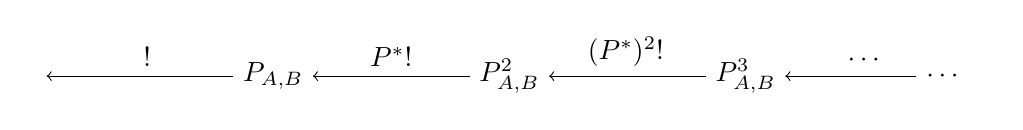
\begin{tikzpicture}[scale=4]
      \node (A) [] {$\unittype$};

      \node (B) [xshift=2cm, right of=A] {$\apply{P_{A,B}}{\unittype}$};

      \node (C) [xshift=2cm, right of=B] {$\apply{P_{A,B}^2}{\unittype}$};

      \node (D) [xshift=2cm, right of=C] {$\apply{P_{A,B}^3}{\unittype}$};

      \node     [xshift=2cm, right of=D, color=white] {$\cdot$};
      \node (E) [right of=D, xshift=1.5cm] {$\cdots$};

      \draw[->] (B) edge (A) node [above, xshift=-1.6cm] {$!$};
      \draw[->] (C) edge (B) node [above, xshift=-1.5cm] {$\apply{P^*}{!}$};
      \draw[->] (D) edge (C) node [above, xshift=-1.52cm] {$\apply{(P^*)^2}{!}$};
      \draw[->] (E) edge (D) node [above, xshift=-1cm] {$\cdots$};
      % \draw (A) edge [in=-60,out=-20,loop] node[below] {$e$} (A);
    \end{tikzpicture}
  \end{center}
  where $P_{A,B}$ is the polynomial functor associated to a given signature and
  $P_{A,B}^i$ represents the $i$\textsuperscript{th} repeated application of $P_{A,B}$.
  The M-type associated to $\dpair{A}{B}$ is the limit of this diagram.
\end{example}

Recall that the standard limit (\cref{def:standard-limit}) is constructed using
universal quantification over the edges between two given vertices. Since we
know that there is at most one edge between any two vertices in this graph,
we can simplify the limits of chain diagrams (this simplification corresponds to
\cite[Definition 9]{non-wellfounded}).

\begin{lemma}[\unimathname{M.Chains.standard\_limit\_of\_cochains}]
  For a cochain $\dpair{X}{π}$, there is a simplifying equivalence
  \begin{align*}
    \apply{\Stdlim}{\dpair{X}{π}}
    &\jdeq \∑{x:\∏{v:G_0}{\apply{D}{v}}}
      {\∏{u,v:G_0}{\∏{e:\appply{G_1}{u}{v}}{\propeq{}{\appply{D}{e}{(\apply{x}{u})}}{\apply{x}{v}}}}} \\
    &\jdeq \∑{x:\∏{v:\ℕ}{X_v}}
      {\∏{u,v:\ℕ}{\∏{e:\propeq{}{\apply{\suc}{v}}{u}}{\propeq{}{\appply{D}{e}{(\apply{x}{u})}}{\apply{x}{v}}}}} \\
    &\weqsign
        {\∑{x:\∏{n:\ℕ}{X_n}}{\∏{n:ℕ}{\propeq{}{\appply{D}{(\refl{\apply{\suc}{n}})}{(\apply{x}{u})}}}{\apply{x}{v}}}}
  \end{align*}
\end{lemma}

\begin{lemma}[\unimathname{M.Chains.shifted\_limit}]
  \label[lemma]{lemma:shifted-limit}
  Let $\dpair{X}{π}$ be a chain. The \define{shifted chain} $\dpair{X'}{π'}$
  is defined by $X'_n\defeq X_{\apply{\suc}{n}}$ and $π'_n\defeq π_{\apply{\suc}{n}}$.
  The standard limits of these chains are equivalent.
\end{lemma}

This is a proof by the algebra of types up to weak equivalence, i.e.\
facts like if $B$ is contractible then $\weq{A}{A×B}$. 

\subsection{Future directions}
\label{subsec:future-directions}

The goal was to establish the following:

\begin{theorem}
	There is a unique terminal coalgebra for any signature $\dpair{A}{B}$.
  Specifically, the following type is contractible:
  \begin{equation*}
    \apply{\Final}{\dpair{A}{B}}\defeq
    \∑{(X,α):\apply{\Coalgtype}{\dpair{A}{B}}}{
      \∏{(Y,β):\apply{\Coalgtype}{\dpair{A}{B}}}
        {\apply{\isContr}{\dpair{Y}{β}⇒\dpair{X}{α}}}
    }
  \end{equation*}
\end{theorem}

Unfortunately, this is not yet proved in \UniMath{}.
There was no fundamental obstacle to its formalization, merely a lack of time.
The main prerequisites yet to be completed are
\cref{lemma:fiber-initiality-nat} and the following lemma
(\cite[Lemma 13]{non-wellfounded}):

\begin{lemma}
	Polynomial functors commute with limits of chains.
  Let $\dpair{L}{p}$ be the limit of $\dpair{X}{π}$, and define
  $\dpair{\apply{P}{X}}{\apply{P^*}{π}}$ by $(\apply{P}{X})_n\defeq \apply{P}{X_n}$
  and similarly for $\apply{P^*}{π}$. Then there is an equivalence
  \begin{equation*}
    \weq{\apply{P}{L}}{\apply{\Stdlim}{\dpair{\apply{P}{X}}{\apply{P^*}{π}}}}
  \end{equation*}
\end{lemma}

If the above were to be proved, it would remain only to show that the universal
property of the limit, when applied to the limit $L$ of the diagram constructed
in \cref{ex:termcochain}, is equivalent to the statement that $L$ is a terminal
coalgebra for $\dpair{A}{B}$. The equivalence $w:\weq{L}{\apply{P}{L}}$
(\cref{lemma:shifted-limit}) gives $L$ the structure of a coalgebra.

To show that $\dpair{L}{w}$ is terminal, \cite{non-wellfounded} doesn't explicitly
construct a coalgebra homomorphism to it from an arbitrary coalgebra
$\dpair{Y}{β}$, but rather uses the algebra of types up to weak equivalence to
show
\begin{equation*}
  \weq{\paren{\dpair{Y}{β}⇒\dpair{L}{w}}}{\unittype}.
\end{equation*}

\end{document}